%!TEX root = report.tex
\exercise{Highboost filtering}
\setcounter{subsection}{0}

Sometimes it is desirable to highlight high-frequency components in an image without eliminating the low-frequency components.
One way to do this is by using a technique called highboost filtering. This technique works by first blurring the image, then subtracting the blurred image from the original image - the result of this operation is called the mask - and then adding the mask to the original image.
Now edges are highlighted while retaining the same information about low-frequency components. 
\subsection{Implementation}
We have implemented the highboost filter in the function \texttt{IPhighboost}. We have set the blur mask to the same mask as in figure 3.32(a) as in the book, or as in table~\ref{tbl:mask}.
\begin{table}[!htb]
\begin{center}
$\frac{1}{9}$
\begin{tabular}{|c|c|c|}\hline
1 & 1 & 1 \\ \hline
1 & 1 & 1 \\ \hline
1 & 1 & 1 \\ \hline
\end{tabular}
\caption{The gaussian mask used for blurring}
\label{tbl:mask}
\end{center}
\end{table}
The following code implements the highboost filter operation (with IPfilter the same function as in the previous lab assignment):
\matlabexternal{IPhighboost.m}
When tested on the image "dipxetext.tif" the output for $k = 4.5$ gives the result of image~\ref{fig:dipxe}.
This is to our opinion the closest approximation of image 3.40(e) in the book.

\subsection{Negative values}
If an image \verb f  contains only positive values it is possible that the output image \verb g  contains negative values.
Consider the image described in table~\ref{tbl:inImage}. This image clearly contains only positive values. However, if is image is processed using \texttt{IPhighboost} with $k \geq 0.13$ the output image \verb g  will contain a negative value as table~\ref{tbl:outImage} illustrates.
We presume the minimal value of $k$ where negative values occur in the output image has a relation with the minimal value that occurs in the input image but we could not find strong evidence what this relation is. 

\begin{figure}[h]
 \centering
 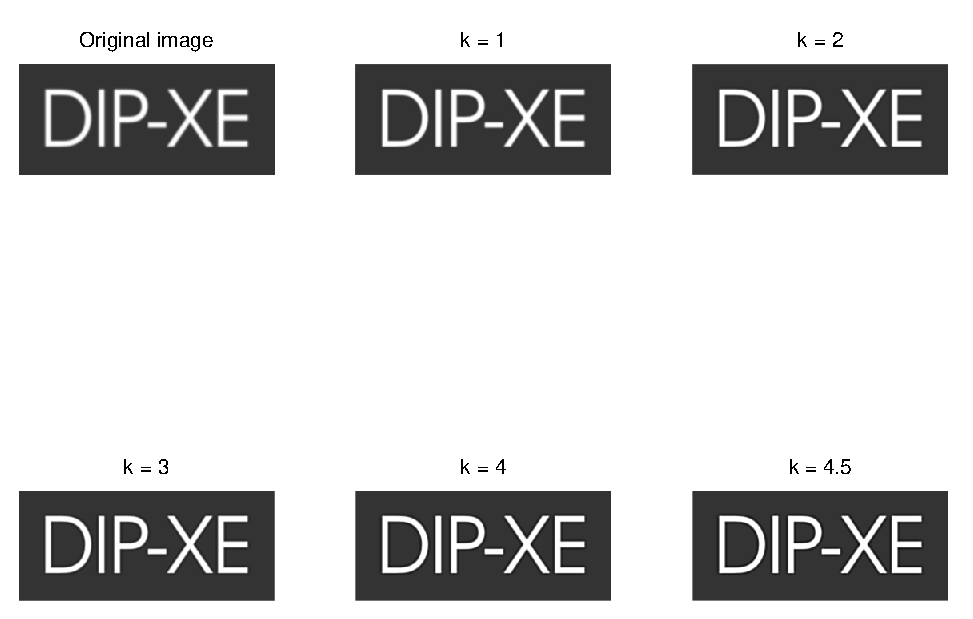
\includegraphics{dipxe.eps}
 \caption{Testing the highboost filter for several options of $k$. The image with $k = 4.5$, bottom-right, is the closest to image 3.40(e) in the book.}
 \label{fig:dipxe}
\end{figure}
\begin{table}[h]
  \begin{minipage}[b]{.5\linewidth}
    \centering
    \begin{tabular}{|c|c|c|}\hline
    1 & 1 & 1 \\ \hline
    1 & 0.1 & 1 \\ \hline
    1 & 1 & 1 \\ \hline
    \end{tabular}
    \subcaption{Input image}
    \label{tbl:inImage}
  \end{minipage}
  \hfill
  \begin{minipage}[b]{.5\linewidth}
    \centering
    \begin{tabular}{|c|c|c|}\hline
      1.3278 & 1.2167 & 1.3278 \\ \hline
      1.2167 & -0.3000 & 1.2167 \\ \hline
      1.3278 & 1.2167 & 1.3278 \\ \hline
    \end{tabular}
    \subcaption{Output image containing a negative value}
    \label{tbl:outImage}
  \end{minipage}
  \caption{The in- and output images for \texttt{IPhighboost}. It is clear that the output image contains negative values.}
  \hfill
\end{table}
\clearpage